
\section{Структура и принцип работы исследуемого пневмопривода}\label{sec:ch2/sec1}
Исследуемый электропневматический привод включает пневматический цилиндр двустороннего действия
c односторонним штоком и четыре двухпозиционных распределителя.
Цилиндр содержит две рабочие полости, разделенные поршнем.

Ключевой особенностью привода является конфигурация распределителей.
К каждой полости цилиндра подключены два независимых распределителя:
один для подачи сжатого воздуха из магистрали, другой для выхлопа в атмосферу.
Такая конфигурация обеспечивает гибкое управление потоками воздуха в обеих полостях цилиндра.

\begin{figure}[h]
    \centerfloat{
        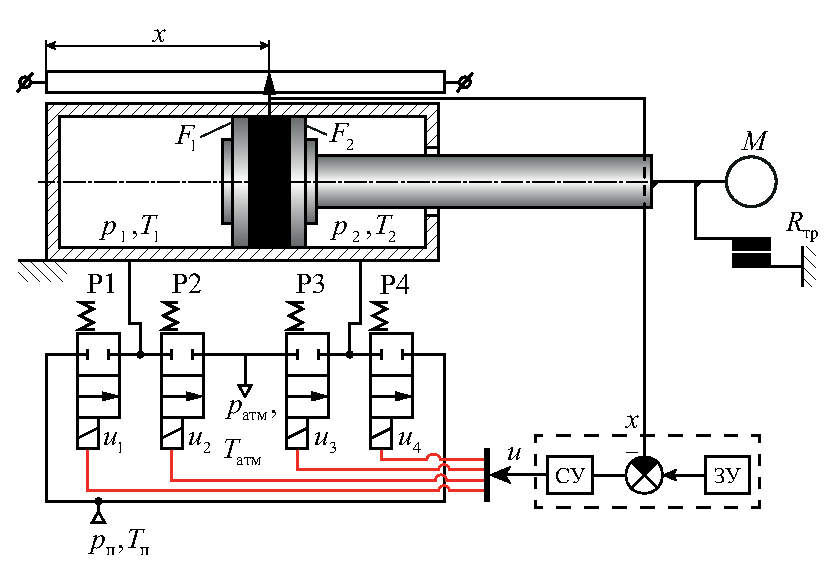
\includegraphics[]{part2/расчетная_схема_привода.eps}
    }
    \caption{Принципиальная пневматическая схема исследуемого привода}
    \label{fig:ch2/pneumatic_actuator_scheme}
    
\end{figure}

Каждый распределитель имеет два дискретных состояния: открыто и закрыто.
Общее количество возможных комбинаций состояний распределителей
определяется формулой:
\begin{equation}
    N = 2^k,
\end{equation}
где $N$ - число комбинаций, $k$ - количество распределителей.

Для рассматриваемой системы с четырьмя распределителями:
\begin{equation}
    N = 2^4 = 16.
\end{equation}

Таким образом, система имеет 16 дискретных состояний, что обеспечивает широкие возможности
управления при сохранении относительной простоты конструкции.

Система управления генерирует дискретные сигналы для активации
электромагнитных клапанов распределителей. Обратная связь по положению реализуется посредством датчика линейного перемещения на штоке цилиндра. 

Использование дискретных распределителей вместо пропорциональных, как было сказано ранее,
снижает стоимость системы, однако требует разработки более сложных
алгоритмов управления для компенсации нелинейного характера коммутации пневматических линий.